%%%%%%%%%%%%%%%%%%%%%%%%%%%%%%%%%%%%%%%%%%%%%%%%%%%%%%%%%%%%%%%%%%%%%%%
% This document is based on the template: Large Colored Title Article %
%                                         Version 1.1 (25/11/12)      %
%                                                                     %
% The template was downloaded from: http://www.LaTeXTemplates.com     %
%                                                                     %
% Original author:                                                    %
% Frits Wenneker (http://www.howtotex.com)                            %
%                                                                     %
% License:                                                            %
% CC BY-NC-SA 3.0 (http://creativecommons.org/licenses/by-nc-sa/3.0/) %
%                                                                     %
% Author of this version:                                             %
% Laura M. Castro (http://www.madsgroup.org/staff/laura)              %
%                                                                     %
% Original licensing terms are maintained                             %
%%%%%%%%%%%%%%%%%%%%%%%%%%%%%%%%%%%%%%%%%%%%%%%%%%%%%%%%%%%%%%%%%%%%%%%

%----------------------------------------------------------------------------------------
%	PACKAGES AND OTHER DOCUMENT CONFIGURATIONS
%----------------------------------------------------------------------------------------

\documentclass[DIV=calc,paper=a4,fontsize=11pt,onecolumn]{scrartcl}	 % A4 paper and 11pt font size

\usepackage[spanish]{babel} % Galician language/hyphenation
\usepackage[utf8]{inputenc}
\usepackage[protrusion=true,expansion=true]{microtype} % Better typography
\usepackage{amsmath,amsfonts,amsthm} % Math packages
\usepackage[svgnames]{xcolor} % Enabling colors by their 'svgnames'
\usepackage[hang,small,labelfont=bf,up,textfont=it,up]{caption} % Custom captions under/above floats in tables or figures
\usepackage{booktabs} % Horizontal rules in tables
\usepackage{fix-cm}	 % Custom font sizes - used for the initial letter in the document

\usepackage{sectsty} % Enables custom section titles
\allsectionsfont{\usefont{OT1}{phv}{b}{n}} % Change the font of all section commands

\usepackage{fancyhdr} % Needed to define custom headers/footers
\pagestyle{fancy} % Enables the custom headers/footers
\usepackage{lastpage} % Used to determine the number of pages in the document (for "Page X of Total")

% Headers - all currently empty
\lhead{}
\chead{}
\rhead{}

% Footers
\lfoot{\textsc{vvs-monitorización-probas}}
\cfoot{}
\rfoot{\footnotesize Páxina \thepage\ de \pageref{LastPage}} % "Page 1 of 2"

\renewcommand{\headrulewidth}{0.0pt} % No header rule
\renewcommand{\footrulewidth}{0.4pt} % Thin footer rule

\definecolor{UDC}{RGB}{206,0,124}
\definecolor{DarkUDC}{rgb}{0.75,0.75,0.75}
\definecolor{LightUDC}{RGB}{128,128,128}

\usepackage{lettrine} % Package to accentuate the first letter of the text
\newcommand{\initial}[1]{ % Defines the command and style for the first letter
\lettrine[lines=3,lhang=0.3,nindent=0em]{
\color{UDC}
{\textsf{#1}}}{}}

%----------------------------------------------------------------------------------------
%	TITLE SECTION
%----------------------------------------------------------------------------------------

\usepackage{titling} % Allows custom title configuration

\newcommand{\HorRule}{\color{UDC} \rule{\linewidth}{1pt}} % Defines the pink horizontal rule around the title

\pretitle{\vspace{-30pt} \begin{flushleft} \HorRule \fontsize{20}{20} \usefont{OT1}{phv}{b}{n} \color{DarkUDC} \selectfont} % Horizontal rule before the title

\title{MONITORIZACIÓN DE PROBAS} % Your article title

\posttitle{\par\end{flushleft}\vskip 0.5em} % Whitespace under the title

\preauthor{\begin{flushleft}\large \lineskip 0.5em \usefont{OT1}{phv}{b}{sl} \color{DarkUDC}} % Author font configuration

\author{Título proxecto: Suite de Probas (VVS) \\
        Ref. proxecto: Equipo 8 \\
        Autores: Eloy Naveira Carro, Alejandro López Sánchez, Adrián Leira Carro, Andrea Ardións Baña}

\postauthor{\footnotesize \usefont{OT1}{phv}{m}{sl} \color{Black} % Configuration for the institution name
\par\end{flushleft}\HorRule} % Horizontal rule after the title

\date{\sffamily Validación e Verificación de Software} % Add a date here if you would like one to appear underneath the title block

%----------------------------------------------------------------------------------------

\usepackage{graphicx}
\usepackage{hyperref}
\hypersetup{colorlinks=true,
            allcolors=UDC}

\usepackage{array}
\usepackage{colortbl}

%----------------------------------------------------------------------------------------

\newcommand{\hint}[1]{\begin{quote}\itshape #1 \end{quote}}

%----------------------------------------------------------------------------------------

\begin{document}

\maketitle % Print the title
\thispagestyle{fancy} % Enabling the custom headers/footers for the first page 

%----------------------------------------------------------------------------------------
%	ABSTRACT
%----------------------------------------------------------------------------------------

\vspace*{1cm}

\begin{center}
\small \sffamily
\begin{tabular}{c|c|c}
Data de aprobación & Control de versións & Observacións \\  \hline 
16/12/2015 & 1.0 & \\ \hline
& & \\ \hline
& & \\
\end{tabular}
\end{center}

\clearpage

%----------------------------------------------------------------------------------------
%	ARTICLE CONTENTS
%----------------------------------------------------------------------------------------

\section{Contexto}

Neste documento recollemos unha suite de probas que aplicamos ao noso proxecto pra que gañase consistencia e estabilidade de cara a un futuro, xa que seguimos a filosofía de que "mais tempo en probas, menos tempo en mantemento". \\
	
	Elaboramos un plan de probas, unha suite de probas, co obxetivo de que ofreza a máxima confianza e así ter unha aplicación funcional, sen erros, e no caso de telos, ser conscientes e saber qué camiño tomar pra resolvelos.

\section{Estado actual}

O estado do proxecto antes de iniciar esta suite de probas era incerto, posto que só contábamos con probas de JUnit. Pra resolvelo, e mellorar a calidade das probas e do proxecto, decidimos tomar os seguintes camiños, e elaborar probas seguindo estas ferramentas de monitorización de probas: 

  \begin{itemize}
  	\item Ferramentas para automatizar a execución de probas dinámicas:
	  	\subitem JUnit: antes de empezar a elaborar esta suite de probas, xa tiñamos test con JUnit. Permítenos elaborar probas unitarias e ver se os métodos se comportan da forma esperada. 
	  	
  	\item Ferramentas para automatizar a xeración de datos en execución de probas dinámicas:
	  	\subitem QuickCheck: está ferramenta úsase, como di máis arriba, para a xeración aleatoria de casos de proba.
	  	
	  	
	  	Fixéronse test de este tipo en tódolos métodos das clases test do sistema.
	  	Consiste básicamente en implementar un bucle en cada caso de proba que xere elementos aleatorios, xa sea usando xeradores proporcionados pola ferramente, ou ben, creando uns personalizados. Fixéronse probas con estes dous tipos de xeradores.
	  	
	  	
	  	A continuación móstrase un exemplo do funcionamento do caso de proba:
	  	
	  	\includegraphics[width=13cm]{Imagenes/quickcheck1.png}
	  	
	  	
	  	Como pode observarse, neste caso úsase un xerador de strings proporcionado pola ferramenta.
	  	
	  	
	  	A continuación móstrase un exemplo no que se usa un xerador personalizado:
	  	
	  	\includegraphics[width=13cm]{Imagenes/quickcheck2.png}
	  	
	  	
	  	E a implementación do xerador:
	  	
	  	\includegraphics[width=13cm]{Imagenes/quickcheck3.png}
	 
		 
  	\item Ferramentas para automatizar a xeración e execución de probas dinámicas:
	  	
	  	\subitem GraphWalker é unha libraría de Java para automatizar a xeración e execución de probas dinámicas. A idea xeneral consiste no deseño do diagrama de estados do sistema para logo mediante unhas probas verificar o funcionamento contra este diagrama. 
	  	
	  	Unha vez realizado o diagrama de estados situase dentro do proxecto e a continuación xérase a interfaz que hai que implementar para as probas. Non chegamos a completar o uso desta ferramenta porque encontrámonos con numerosos erros que non soubemos arranxar.
	  	
	  	
	  	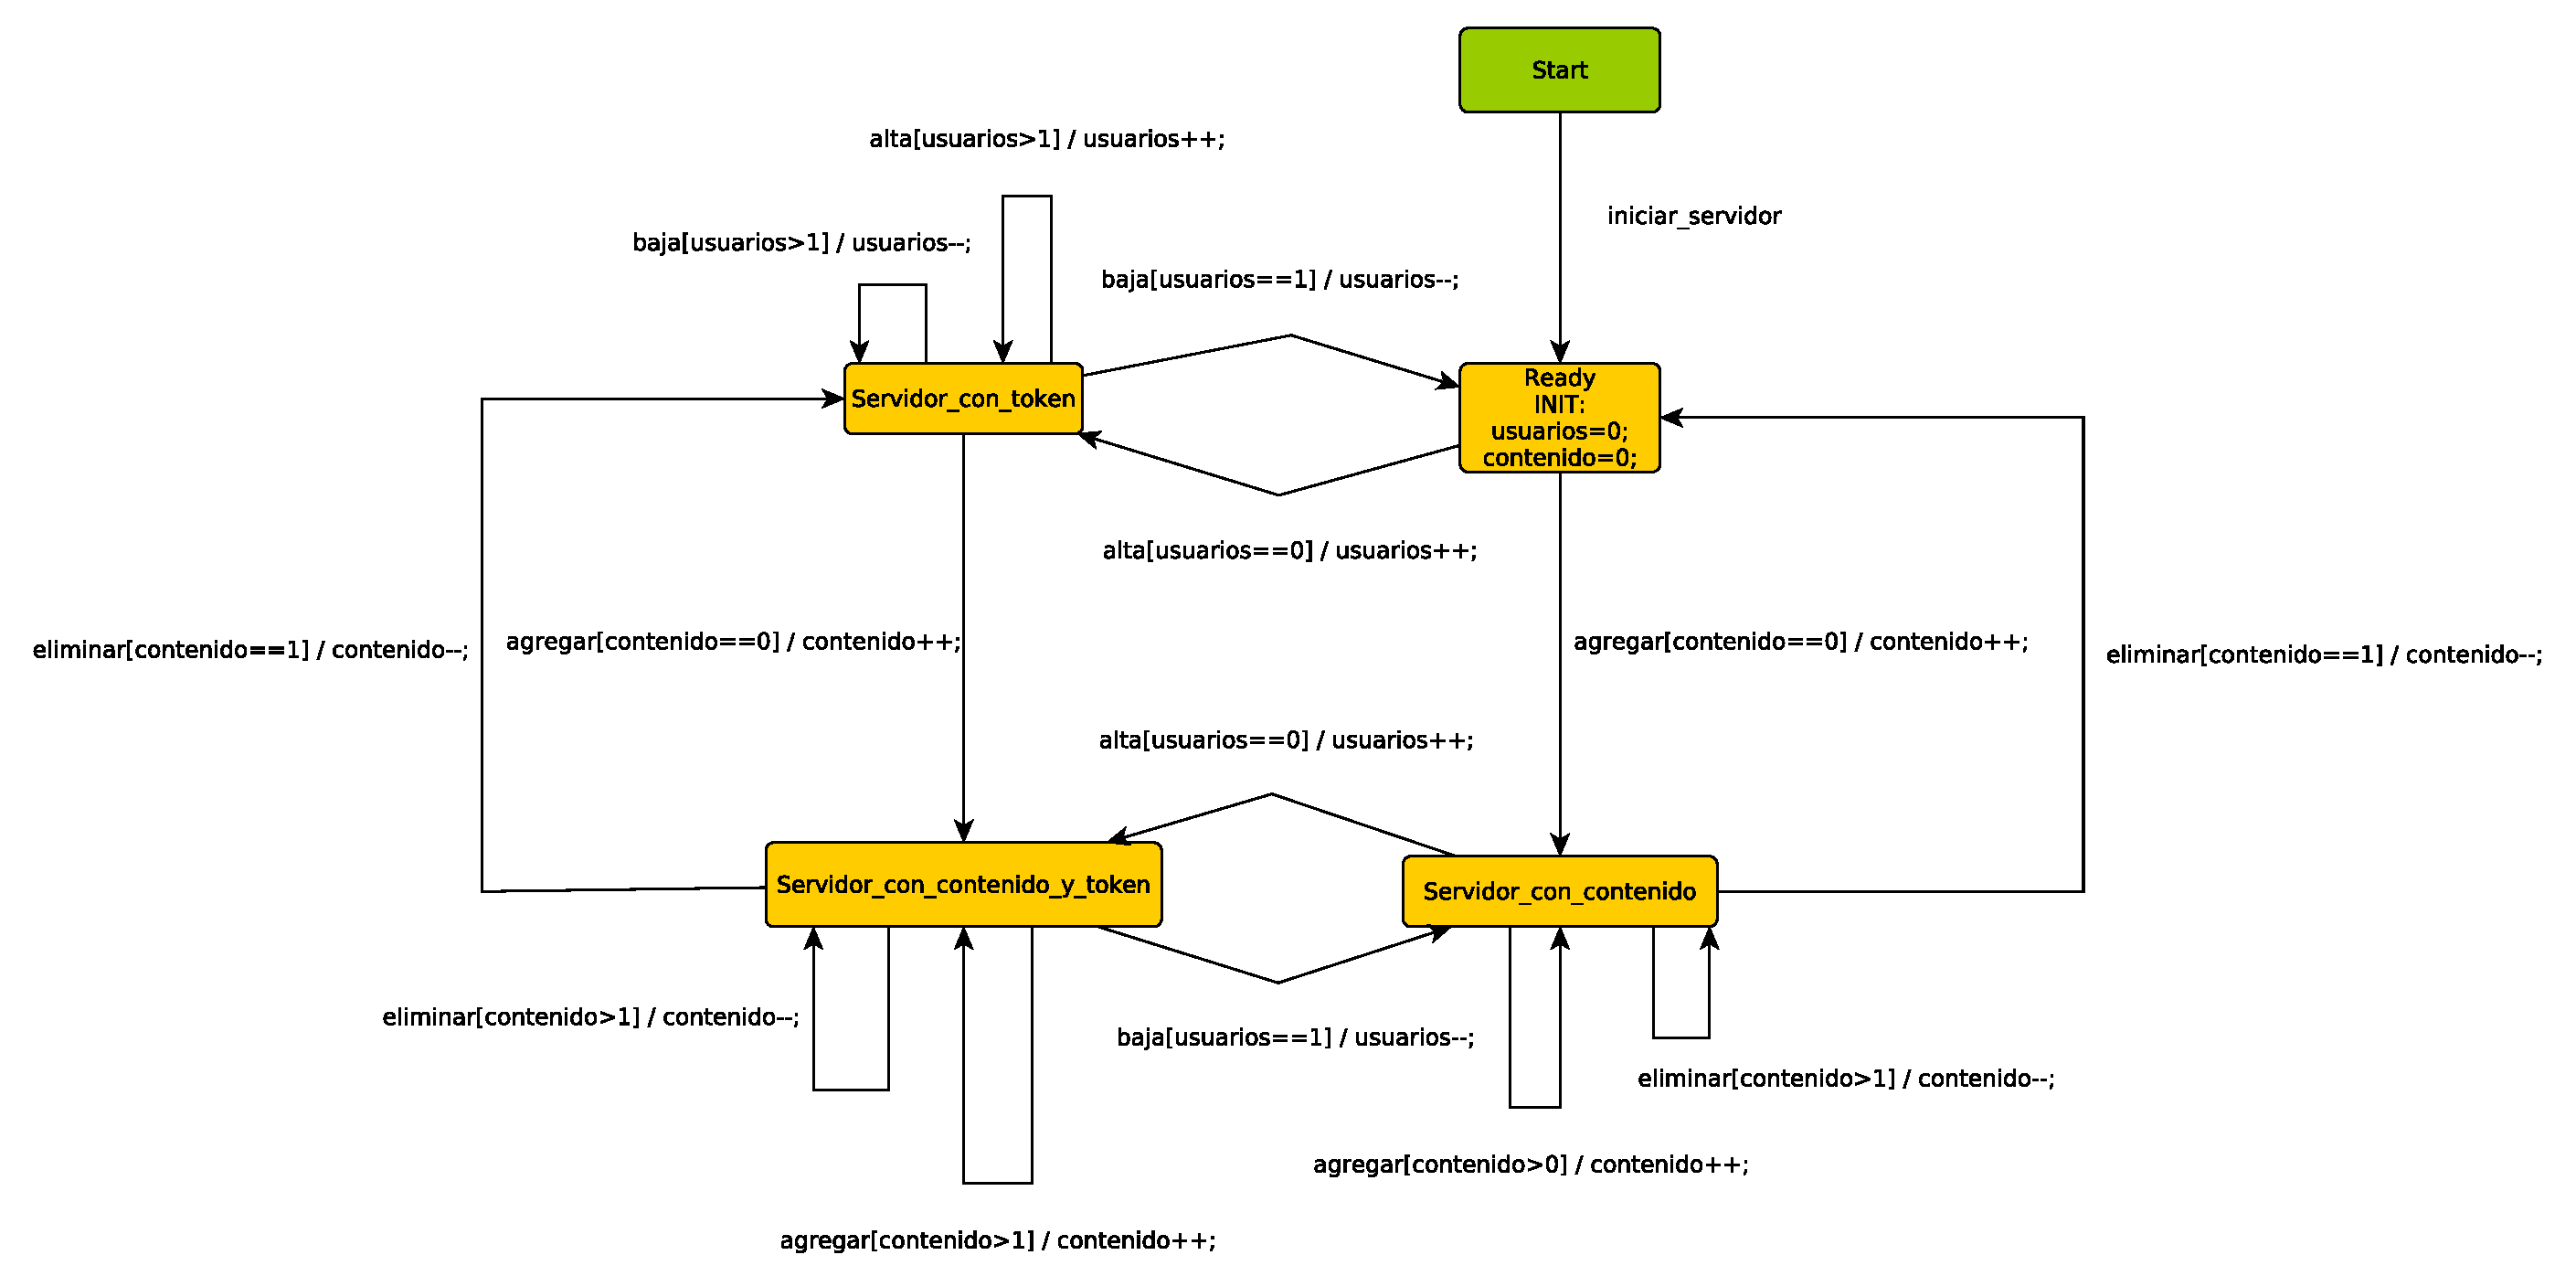
\includegraphics[width=13cm]{Imagenes/servidor.pdf}
	  	
	  	\includegraphics[width=13cm]{Imagenes/interfazGW.png} 
	  	
	  	
	  	
	\item Ferramentas para validación da calidade das probas:
		\subitem Cobertura: contar con Cobertura é crucial pra saber a calidade das probas, pra saber con exactitude a cantidade de código que estamos probando cos test. \\
		
		Este foi o informe inicial tras a primeira proba de Cobertura:\\
		
		\includegraphics[width=15cm]{Imagenes/cobertura-inicio.jpg}
		
		Este é o informe final:\\
		
		\includegraphics[width=15cm]{Imagenes/cobertura-final.jpg} \\
		
		Estos datos mostran que ao principio as probas non pasaban por todo o código, pero o mellorar a calidade das mesmas, agora atopámonos con mellores resultados. Tivemos que optar por test de mellor calidade, que abarcasen as máximas líneas de código posibles.\\
		
		E isto non e todo, porque cobertura axudounos a darnos conta de que tiñamos métodos sen testear, e ademáis, de malas prácticas ahora de deixar métodos dunha Interface sen implementación. \\
		
		O ideal, e acadar mais dun 80 de porcentaxe en cobertura, e iso é o que conseguimos.\\
		
		\subitem PIT: Mutation Testing axudaranos a mellor a calidade das probas atopadas, con pistas pra que as melloremos. E unha maneira de resolver erros que coas probas unitarias non atoparíamos nunca, posto que lle da a volta a situación pra analizar o código. O obtetivo, que todas as mutacions rematen en KILLED.\\
		
		A primeira vez que o pasamos (depois de amañar as carencias de Cobertura) atopámonos cos seguintes resultados: \\
		
		\includegraphics[width=15cm]{Imagenes/pit-inicio.jpg} \\
		
		Centrándonos na clase Emisora, vemonos que seguindo unha das recomendacions de PIT a mutación ada un 16/16. \\
		
		\begin{center}
		\includegraphics[width=8cm]{Imagenes/cambios-pit.jpg}
		\end{center}
		
		Tras amañar a implementación de Emisora, o resultado tras isto mellora: \\
		
		\includegraphics[width=15cm]{Imagenes/pit-medio.jpg} \\
		
		E por último, chegamos a conclusión de que aplicando outras ferramentas de proba, podemos conseguir acadar mellores resultados pasando de novo PIT-Mutation, pasando dun 85 de porcentaxe e 69 respectivamente, a 93 e 75, que é mais aceptable tengo en conta como é PIT.  \\
		
		\includegraphics[width=15cm]{Imagenes/pit-final.jpg} \\
		
  	\item Ferramentas para facilitar as probas dinámicas de unidade:
	  
	  \subitem Mockito: é unha libraría de Java (baseado en EayMock) para a creación de Mocks ou obxetos simulados moi empregados en probas unitarias en TDD (Test Driven Development), que é unha práctica de programación baseada na creación de probas primeiro. Mockito creouse co fin de correxir algúns dos problemas de EasyMock.
	  
	  Na nosa práctica simulamos o comportamento das implementacións da interfaz Contenido para realizar as probas do Servidor.
	  
	  A aplicación básica desta ferramenta consiste, en primeiro lugar, na declaración das clases mock e as suas cláusulas de comportamento, ou stubs, que definen os valores que teñen que devolver as distintas funcións ou métodos desa clase.
	  \\
	  \includegraphics[width=15cm]{Imagenes/mocks.png} \\
	  \\
	  \includegraphics[width=15cm]{Imagenes/stubs.png} \\
	  \\
	  
	  Unha vez preparados os mocks e definidos os stubs de cada un, pasamos a implementación das probas. Nalgúns casos das probas empregamos a cláusula verify que comproba a execución do método sinalado, e incluso o número de veces que se executou.
	  \\
	  \includegraphics[width=15cm]{Imagenes/verify.png} \\
	  \\
	  
	  Durante a realización destas probas atopouse un erro nas dúas implementacións do Servidor. O erro consistía no caso de que se buscase os anuncios contidos nas emisoras non encontraba ningún. Este erro debeuse a que non se comprobou este caso nas probas feitas previamente.
	  
	\item Ferramentas para probas non funcionais:
		\subitem JETM: é unha librería que se utiliza para axudar a localizar problemas de rendemento en aplicacións Java. \\
		
		Ten un uso relativamente sinxelo. Consiste en colocar puntos de monitorización nos métodos nos que se queira comprobar o rendemento, e na clase test chamar a un monitor que mostre os resultados desa monitorización. \\
		
		Decidiuse comprobar só o rendemento do Servidor, xa que o de respaldo é similar, e as implementacións de Contenido son bastante triviais. \\ 
		
		Móstrase a continuación os resultados do monitor no Servidor:
		
		\includegraphics[width=13cm]{Imagenes/jetm.png} \\
  	  \item Ferramentas para probas estruturais/estáticas:
	  	  \subitem PMD: esta ferramenta permítenos darnos conta das malas decisións que tomamos a hora de programar. Atopámonos con todo tipo de recomendacions pra mellorar o código, como pode ser na clase Emisora que é a que tomamos de exemplo, e coa que conseguimos acadar uns bos resultados tras a aplicación desta ferramenta. \\
	  	  
	  	  Aplicamos decisións como convertir clases a final, ou mellorar a maneira de facer as probas empregando assertEquals mellor que assertTrue e asserteFalse. \\
	  	  
	  	  Este é o resultado de PMD antes de amañar Emisora: \\
	  	  
	  	  \includegraphics[width=15cm]{Imagenes/test-pmd-antes-emisora.png} \\
	  	  
	  	  Este é o resultado de PMD despois de amañar Emisora: \\
	  	  
	  	  \includegraphics[width=15cm]{Imagenes/test-pmd-despues-emisora.png} \\
	  	  
	  	  Como podemos ver, os resultados son moito mellores, demostrando que non só podemos deixarnos levar por probas como JUnit, senon tamen acadar unha boa suite de probas pra analizar cantos mais problemas mellor.
	  	  
	  	  \subitem FindBugs: con esta herramienta o que se querer probar é se hay algún tipo de bug potencial no sistema. Despois de executalo, o resultado é o seguinte:
	  	  
	  	  
	  	  \includegraphics[width=13cm]{Imagenes/findbugs.png}
	  	  
	  	  Con esto sácase en claro que existe un posible bug potencial na clase GenerarToken, pero despois de analizar a clase do erro, se chega á conclusión de que é un erro de encoding, polo que non se considera relevante.
  \end{itemize}

\section{Rexisto de probas}

As causas dos atrasos, debéronse case na súa totalidade a falta de información a hora de preparar o entorno pra executar as probas. Sí e certo que contamos con moita documentación de cada tipo de proba na súa correspondente páxina oficial, pero moitas veces queda un pouco no aire cómo seguir os pasos. E por isto, polo que na súa maioría atopámonos con dúbidas sobre qué pasos seguir, erros tras a execución errónea de probas, pero que co paso do tempo fumos resolvendo sen problemas. \\

O mellor de todo isto sen dúbida, foi darnos conta como co paso do tempo e así que executábamos mais probas, acadábamos mellores resultados e descubríamos mellores formas de facer as cousas que no seu momento se nos pasaran por alto. 

\section{Rexistro de erros}

Non atopamos probas que revelasen incumprimentos nas especificacions, pero sí faltaba algún método que non contempláramos no seu momento.\\

\section{Estatísticas}


  \begin{itemize}
    \item Número de erros encontrados diariamente e semanalmente: a medida que probamos as diferentes ferramentas de monitorización de probas, atopámosnos con erros, pero non erros que foxen en contra da especificacion, senon melloras. \\
    \item Nivel de progreso na execución das probas: o progreso foi progresivo. A execución de determinadas probas levounos a obter test mais precisos e completo, conseguindo unha evolución de probas moi positiva. Pasando por exemplo dun porcentaxe do 60 en cobertura ata mais do 80.  \\
    \item Análise do perfil de detección de erros (lugares, compoñentes, tipoloxía): todos vinculados coa seguridade, visibilidade, algún de rendemento... malas prácticas de programación.\\
    \item Informe de erros abertos e pechados por nivel de criticidade: no seu momento tivemos issues abertas, que xiraron en torno a seguridade e visibilidade de cada un dos componentes. \\
    \item Avaliación global do estado de calidade e estabilidade actuais: mellorable, pero estable, funcional e moito mellor que cando empezamos coa suite de probas. \\
  \end{itemize}

\section{Outros aspectos de interese}

Cada proba foi crucial para acadar unha mellor calidade do proxecto. O análise do código con Cobertura axudounos a mellorar a calidade das probas, pero as demáis probas, axudaron a mellor a calidade do proxecto na súa totallidade. \\

Trala execución de quickcheck tampouco se descubriron novos erros. Para o que serviu foi para incrementar en gran medida a confianza na robustez das nosas probas.

\end{document}
